% ------------------------------------------------------------------------------
% TYPO3 CMS 7.6 - What's New - Chapter "In-Depth Changes" (German Version)
%
% @author	Patrick Lobacher <patrick@lobacher.de> and Michael Schams <schams.net>
% @license	Creative Commons BY-NC-SA 3.0
% @link		http://typo3.org/download/release-notes/whats-new/
% @language	German
% ------------------------------------------------------------------------------
% LTXE-CHAPTER-UID:		7229f1b9-b481e9bc-09c46183-a86b6a7e
% LTXE-CHAPTER-NAME:	In-Depth Changes
% ------------------------------------------------------------------------------
% LTXE-SLIDE-START
% LTXE-SLIDE-UID:		d5acb2d2-159a2d7f-6693f827-30cf1736
% LTXE-SLIDE-TITLE:		Bootstrap for Install Tool (1)
% ------------------------------------------------------------------------------

\begin{frame}[fragile]
	\frametitle{Änderungen im System}
	\framesubtitle{Bootstrap für Install Tool(1)}

	\begin{itemize}

		\item Das Install Tool basiert nun komplett auf Bootstrap: Sowohl für die Installation...

			\begin{figure}
				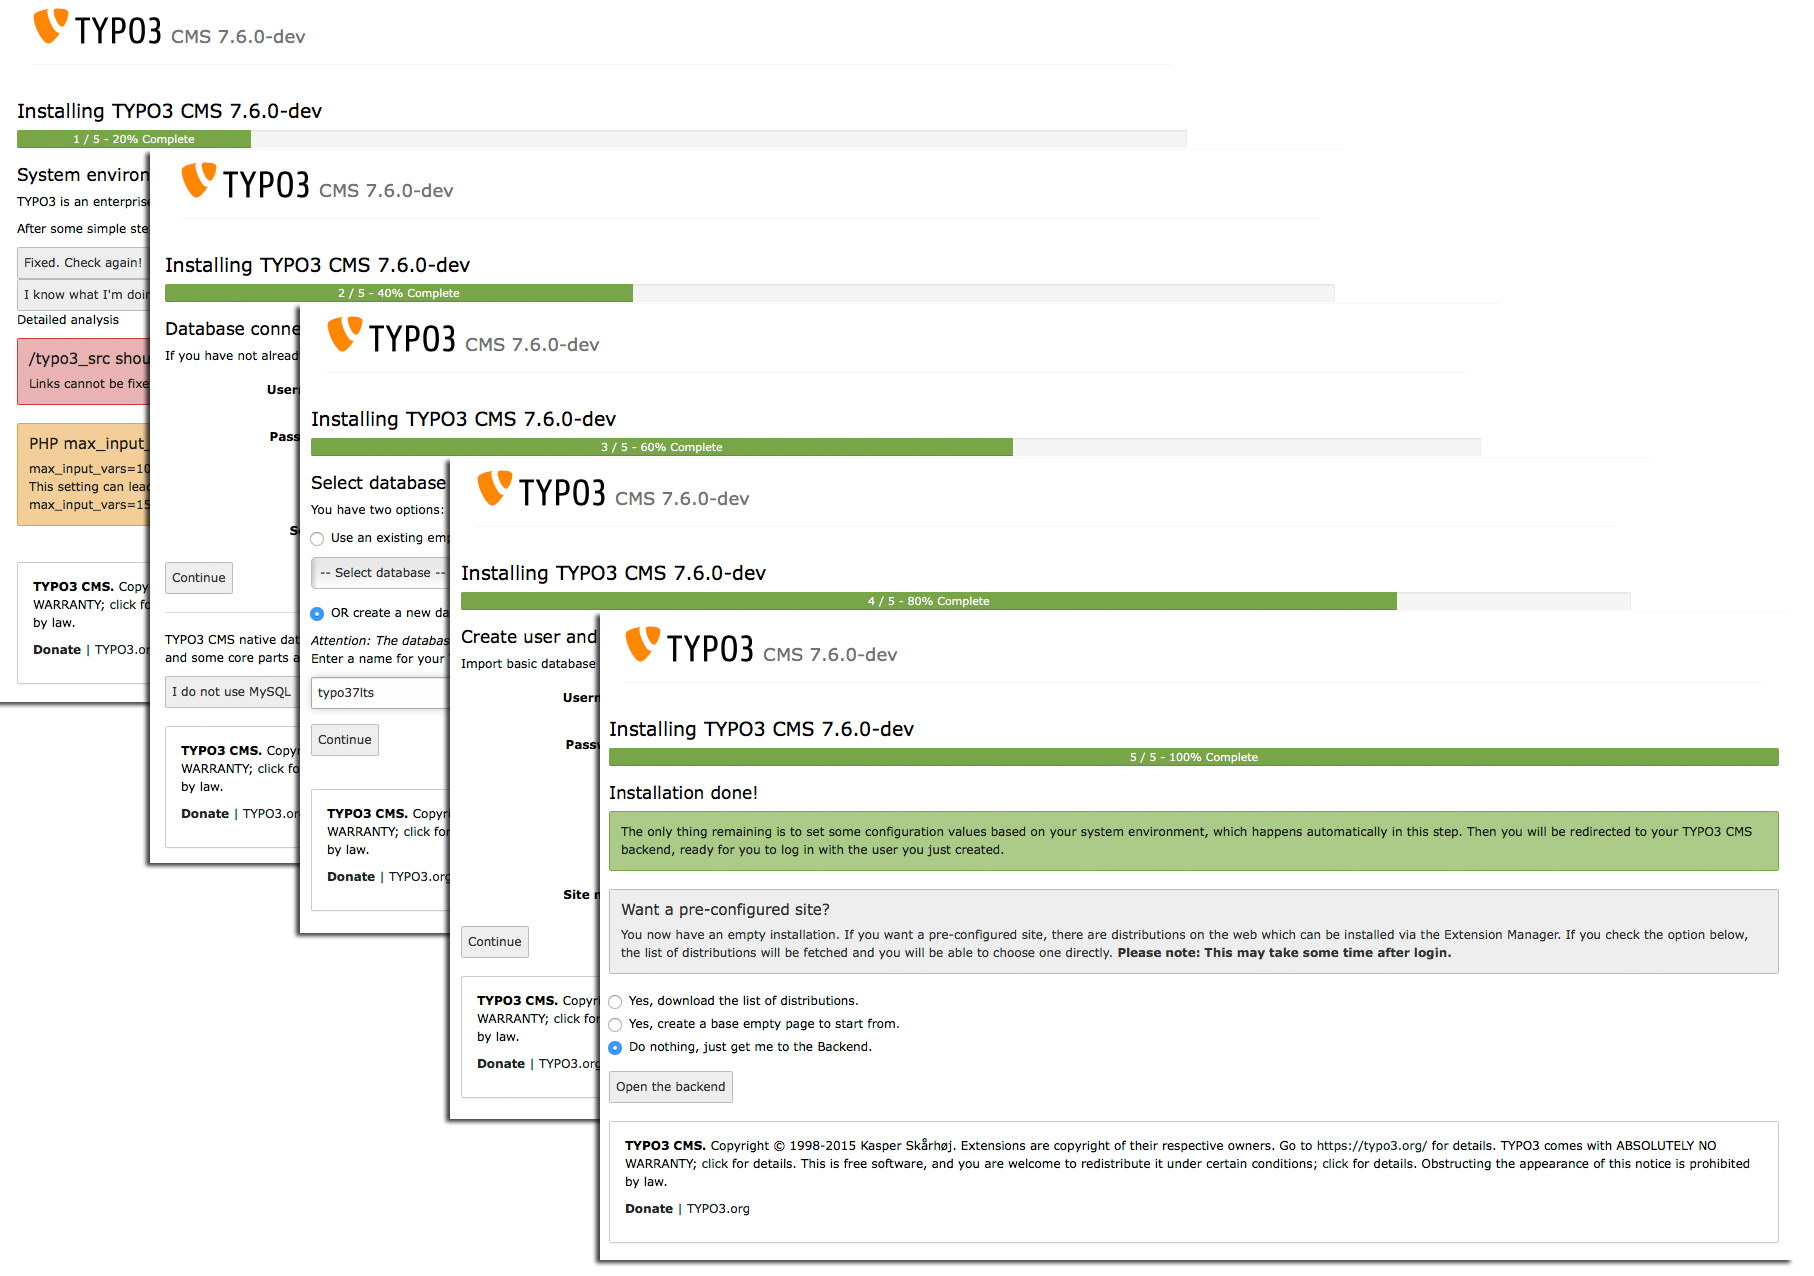
\includegraphics[width=0.7\linewidth]{InDepthChanges/InstallToolBootstrap01.jpg}
			\end{figure}

	\end{itemize}

\end{frame}

% ------------------------------------------------------------------------------
% LTXE-SLIDE-START
% LTXE-SLIDE-UID:		d5acb2d2-159a2d7f-6693f827-30cf1736
% LTXE-SLIDE-TITLE:		Bootstrap for Install Tool (2)
% ------------------------------------------------------------------------------

\begin{frame}[fragile]
	\frametitle{Änderungen im System}
	\framesubtitle{Bootstrap für Install Tool(2)}

	\begin{itemize}

		\item Das Install Tool basiert nun komplett auf Bootstrap: ...wie auch für die Konfiguration

			\begin{figure}
				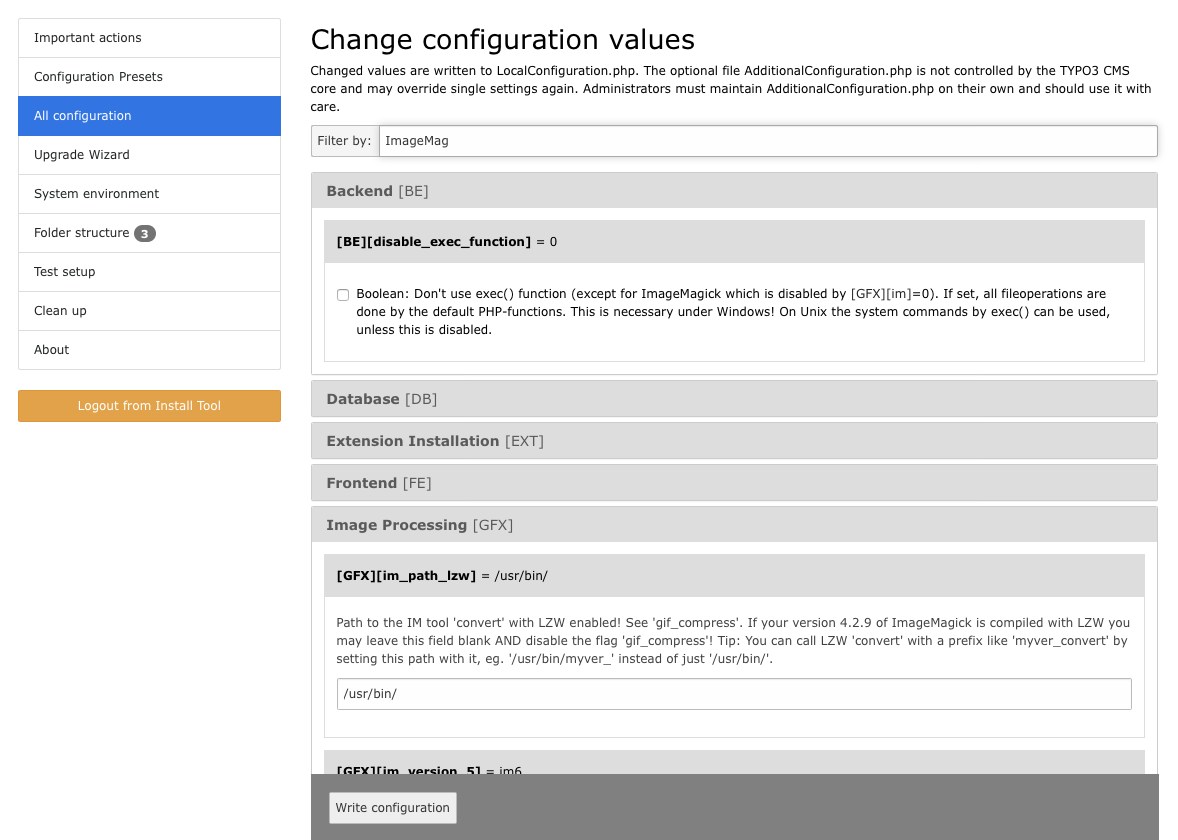
\includegraphics[width=0.7\linewidth]{InDepthChanges/InstallToolBootstrap02.png}
			\end{figure}

	\end{itemize}

\end{frame}

% ------------------------------------------------------------------------------
% LTXE-SLIDE-START
% LTXE-SLIDE-UID:		d5acb2d2-159a2d7f-6693f827-30cf1736
% LTXE-SLIDE-TITLE:		Form protection API for frontend usage
% LTXE-SLIDE-REFERENCE:	Feature-56633-FormProtectionAPIForFrontEndUsage.rst
% ------------------------------------------------------------------------------

\begin{frame}[fragile]
	\frametitle{Änderungen im System}
	\framesubtitle{CSRF Schutz für eigene Plugins}

	% decrease font size for code listing
	\lstset{basicstyle=\tiny\ttfamily}

	\begin{itemize}

		\item Frontend Plugins müssen nun selbst für einen CSRF-Schutz sorgen:

			\begin{lstlisting}
				$formToken = \TYPO3\CMS\Core\FormProtection\FormProtectionFactory::get()->getFormProtection()->generateToken('news', 'edit', $uid);
				if (
				  $dataHasBeenSubmitted
				  && \TYPO3\CMS\Core\FormProtection\FormProtectionFactory::get()->validateToken(
				    \TYPO3\CMS\Core\Utility\GeneralUtility::_POST('formToken'), 'User setup', 'edit')) {
				  // alles in Ordnung
				}
				else {
				  // ungueltiger Token!
				}
			\end{lstlisting}

	\end{itemize}

\end{frame}

% ------------------------------------------------------------------------------
% LTXE-SLIDE-START
% LTXE-SLIDE-UID:		388c7243-b679989c-e2b30dbb-78f1aea4
% LTXE-SLIDE-TITLE:		Added LinkBrowser APIs (1)
% LTXE-SLIDE-REFERENCE:	Feature-66369-AddedLinkBrowserAPIs.rst
% ------------------------------------------------------------------------------

\begin{frame}[fragile]
	\frametitle{Änderungen im System}
	\framesubtitle{Neue Tabs für LinkBrowser (1)}

	% decrease font size for code listing
	\lstset{basicstyle=\tiny\ttfamily}

	\begin{itemize}

		\item Mit diesem Feature kann der LinkBrowser um neue Tabs erweitert werden

		\item Jeder Tab wird über einem sogenannten "LinkHandler" gesteuert, welcher das
			folgende Interface implementieren muss:\newline
			\small
				\texttt{\textbackslash TYPO3\textbackslash CMS\textbackslash Recordlist\textbackslash LinkHandler\textbackslash LinkHandlerInterface}
			\normalsize

		\item Die LinkHandler werden über PageTSconfig registriert:

			\begin{lstlisting}
				file {
				  handler = TYPO3\\CMS\\Recordlist\\LinkHandler\\FileLinkHandler
				  label = LLL:EXT:lang/locallang_browse_links.xlf:file
				  displayAfter = page
				  scanAfter = page
				  configuration {
				    customConfig = passed to the handler
				  }
				}
			\end{lstlisting}

	\end{itemize}

\end{frame}

% ------------------------------------------------------------------------------
% LTXE-SLIDE-START
% LTXE-SLIDE-UID:		dfd89b4b-7b4b816c-e5904ba8-2527339b
% LTXE-SLIDE-TITLE:		Added LinkBrowser APIs (2)
% LTXE-SLIDE-REFERENCE:	Feature-66369-AddedLinkBrowserAPIs.rst
% ------------------------------------------------------------------------------

\begin{frame}[fragile]
	\frametitle{Änderungen im System}
	\framesubtitle{Neue Tabs für LinkBrowser (2)}

	% decrease font size for code listing
	\lstset{basicstyle=\tiny\ttfamily}

	\begin{itemize}

		\item Die Optionen \texttt{displayBefore} und \texttt{displayAfter} geben die Anzeigeposition der Tabs an
		\item Die Optionen \texttt{scanBefore} und \texttt{scanAfter} regeln die Reihenfolge der Ausführung
			\begin{lstlisting}
				$GLOBALS['TYPO3_CONF_VARS']['SC_OPTIONS']['LinkBrowser']['hooks'][1444048118] = [
				  'handler' => \Vendor\Ext\MyClass::class,
				  'before' => [], // optional
				  'after' => [] // optional
				];
			\end{lstlisting}

	\end{itemize}

\end{frame}

% ------------------------------------------------------------------------------
% LTXE-SLIDE-START
% LTXE-SLIDE-UID:		687f24a3-032124a3-7ac41f15-26329962
% LTXE-SLIDE-TITLE:		Module Template API (1)
% LTXE-SLIDE-REFERENCE:	Feature-69814-ModuleTemplateAPI.rst
% ------------------------------------------------------------------------------

\begin{frame}[fragile]
	\frametitle{Änderungen im System}
	\framesubtitle{Neue Module Template API (1)}

	% decrease font size for code listing
	\lstset{basicstyle=\tiny\ttfamily}

	\begin{itemize}

		\item Es wurde eine Module Template API integriert, um die Erstellung der DocHeader zu vereinheitlichen

		\item Beispiel 1: Button hinzufügen

			\begin{lstlisting}
				$openInNewWindowButton = $this->moduleTemplate->getDocHeaderComponent()->getButtonBar()
				  ->makeLinkButton()
				  ->setHref('#')
				  ->setTitle($this->getLanguageService()->sL(
				    'LLL:EXT:lang/locallang_core.xlf:labels.openInNewWindow', TRUE
				    ))
				  ->setIcon($this->iconFactory->getIcon('actions-window-open', Icon::SIZE_SMALL))
				  ->setOnClick($aOnClick);

				$this->moduleTemplate->getDocHeaderComponent()->getButtonBar()
				  ->addButton($openInNewWindowButton, ButtonBar::BUTTON_POSITION_RIGHT);
			\end{lstlisting}
	\end{itemize}

\end{frame}

% ------------------------------------------------------------------------------
% LTXE-SLIDE-START
% LTXE-SLIDE-UID:		1570c8c9-2dfa48e9-058d2d04-bff5465d
% LTXE-SLIDE-TITLE:		Module Template API (2)
% LTXE-SLIDE-REFERENCE:	Feature-69814-ModuleTemplateAPI.rst
% ------------------------------------------------------------------------------

\begin{frame}[fragile]
	\frametitle{Änderungen im System}
	\framesubtitle{Neue Module Template API (2)}

	% decrease font size for code listing
	\lstset{basicstyle=\tiny\ttfamily}

	\begin{itemize}
		\item Beispiel 2: Menü hinzufügen

			\begin{lstlisting}
				$languageMenu = $this->moduleTemplate->getDocHeaderComponent()
				  ->getModuleMenuRegistry()->makeMenu()
				  ->setIdentifier('_langSelector')
				  ->setLabel($this->getLanguageService()->sL(
				    'LLL:EXT:lang/locallang_general.xlf:LGL.language', TRUE
				  ));

				$menuItem = $languageMenu->makeMenuItem()
				  ->setTitle($lang['title'] . $newTranslation)
				  ->setHref($href);

				if((int)$lang['uid'] === $currentLanguage) {
				  $menuItem->setActive(TRUE);
				}

				$languageMenu->addMenuItem($menuItem);
				$this->moduleTemplate->getDocHeaderComponent()->getModuleMenuRegistry()->addMenu($languageMenu);
			\end{lstlisting}
	\end{itemize}

\end{frame}


% ------------------------------------------------------------------------------
% LTXE-SLIDE-START
% LTXE-SLIDE-UID:		df3ea848-d5406e98-edbd6684-485ff477
% LTXE-SLIDE-TITLE:		PSR-7-based Routing for Backend AJAX Requests
% LTXE-SLIDE-REFERENCE:	Feature-69916-PSR-7-basedRoutingForBackendAJAXRequests.rst
% ------------------------------------------------------------------------------

\begin{frame}[fragile]
	\frametitle{Änderungen im System}
	\framesubtitle{PSR-7 Routing für Backend AJAX Requests }

	% decrease font size for code listing
	\lstset{basicstyle=\tiny\ttfamily}

	\begin{itemize}

		\item Um eine Route für einen AJAX-Request zuzufügen, erstellt man eine Datei
			\texttt{Configuration/Backend/AjaxRoutes.php} mit folgendem Inhalt in der eigenen Extension:

			\begin{lstlisting}
				return [
				  // do something
				  'unique_route_name' => [
				    'path' => '/toolcollection/some-action',
				    'target' => \Vendor\Controller\SomeController::class . '::myAction',
				  ]
				];
			\end{lstlisting}

	\end{itemize}

\end{frame}

% ------------------------------------------------------------------------------
% LTXE-SLIDE-START
% LTXE-SLIDE-UID:		cb01cca6-58e91977-d18fa0b3-cba021ab
% LTXE-SLIDE-TITLE:		Introduced two new Hooks for OpenID (getUserRecord)
% LTXE-SLIDE-REFERENCE:	Feature-44127-HooksForOpenIdToAutomaticallyCreateUserAccounts.rst
% ------------------------------------------------------------------------------
\begin{frame}[fragile]
	\frametitle{Änderungen im System}
	\framesubtitle{OpenID Hook \texttt{getUserRecord}}

	% decrease font size for code listing
	\lstset{basicstyle=\tiny\ttfamily}

	Es wurden zwei Hooks zur Verarbeitung von OpenID hinzugefügt (1/2)

		\begin{itemize}

			\item Hook 1:\newline
				\smaller\smaller
					\texttt{\$GLOBALS['TYPO3\_CONF\_VARS']['SC\_OPTIONS']['openid']['getUserRecord']}
				\normalsize

				\begin{itemize}
					\item Modifiziert den Benutzer-Datensatz, nachdem dieser ermittelt wurde, oder:
					\item Legt einen neuen Datensatz an, wenn keine gefunden wurde
					\item Es werden die Parameter \texttt{record}, \texttt{response} und \texttt{authInfo} an den Hook übermittelt
				\end{itemize}

		\end{itemize}

\end{frame}

% ------------------------------------------------------------------------------
% LTXE-SLIDE-START
% LTXE-SLIDE-UID:		ea0bfed8-831666d7-1ba40bb9-7a95723a
% LTXE-SLIDE-TITLE:		Introduced two new Hooks for OpenID (authRequest)
% LTXE-SLIDE-REFERENCE:	Feature-44127-HooksForOpenIdToAutomaticallyCreateUserAccounts.rst
% ------------------------------------------------------------------------------
\begin{frame}[fragile]
	\frametitle{Änderungen im System}
	\framesubtitle{OpenID Hook \texttt{authRequest}}

	% decrease font size for code listing
	\lstset{basicstyle=\tiny\ttfamily}

	Es wurden zwei Hooks zur Verarbeitung von OpenID hinzugefügt (2/2)

		\begin{itemize}

			\item Hook 2:\newline
				\smaller\smaller
					\texttt{\$GLOBALS['TYPO3\_CONF\_VARS']['SC\_OPTIONS']['openid']['authRequest']}
				\normalsize

				\begin{itemize}
					\item Modifiziert den Authentifizierungs-Request bevor dieser abgesendet wird
					\item Damit können z.B. zusätzliche Attribute, wie der Nickname vom OpenID-Server angefordert werden
					\item Es werden die Parameter \texttt{authRequest} und \texttt{authInfo} an den Hook übermittelt
				\end{itemize}

		\end{itemize}

\end{frame}

% ------------------------------------------------------------------------------
% LTXE-SLIDE-START
% LTXE-SLIDE-UID:		115a4459-3653bb99-1680d6ab-d8c3c69b
% LTXE-SLIDE-TITLE:		Hook in BackendUserAuthentication::getDefaultUploadFolder (1)
% LTXE-SLIDE-REFERENCE:	Feature-68895-IntroducedHookInBackendUserAuthenticationgetDefaultUploadFolder.rst
% ------------------------------------------------------------------------------
\begin{frame}[fragile]
	\frametitle{Änderungen im System}
	\framesubtitle{Hooks und Signals (1)}

	% decrease font size for code listing
	\lstset{basicstyle=\tiny\ttfamily}

	\begin{itemize}

		\item Es ist nun möglich, das Verzeichnis, welches von
			\texttt{BackendUserAuthentication::getDefaultUploadFolder()}
			zurückgegeben wird, via Hook zu verändern

		\item Dazu muss folgende Konfiguration in die Datei \texttt{ext\_localconf.php}
			eingetragen werden:

			\begin{lstlisting}
				$GLOBALS['TYPO3_CONF_VARS']['SC_OPTIONS']['t3lib/class.t3lib_userauthgroup.php']
				  ['getDefaultUploadFolder'][] =
				  \Vendor\MyExtension\Hooks\DefaultUploadFolder::class . '->getDefaultUploadFolder';
			\end{lstlisting}

	\end{itemize}

\end{frame}

% ------------------------------------------------------------------------------
% LTXE-SLIDE-START
% LTXE-SLIDE-UID:		d1041967-32814ee3-2172e570-4a6d21bd
% LTXE-SLIDE-TITLE:		Hook in BackendUserAuthentication::getDefaultUploadFolder (2)
% LTXE-SLIDE-REFERENCE:	Feature-68895-IntroducedHookInBackendUserAuthenticationgetDefaultUploadFolder.rst
% ------------------------------------------------------------------------------
\begin{frame}[fragile]
	\frametitle{Änderungen im System}
	\framesubtitle{Hooks und Signals (2)}

	% decrease font size for code listing
	\lstset{basicstyle=\tiny\ttfamily}

	\small Beispiel:\normalsize

		\begin{lstlisting}
			<?php
			namespace Vendor\MyExtension\Hooks;
			use TYPO3\CMS\Core\Authentication\BackendUserAuthentication;
			use TYPO3\CMS\Core\Resource\Folder;

			/**
			 * Class DefaultUploadFolder
			 */
			class DefaultUploadFolder {

			  /**
			   * Get default upload folder
			   * If there is a folder present with the same name as the last part of the table name use that folder.
			   * @param array $params
			   * @param BackendUserAuthentication $backendUserAuthentication
			   * @return Folder
			   */
			   public function getDefaultUploadFolder($params, BackendUserAuthentication $backendUserAuthentication) {
			    [...]
		\end{lstlisting}

\end{frame}

% ------------------------------------------------------------------------------
% LTXE-SLIDE-START
% LTXE-SLIDE-UID:		2f855107-2262065c-c865f953-91b4f0ea
% LTXE-SLIDE-TITLE:		Hook in BackendUserAuthentication::getDefaultUploadFolder (3)
% LTXE-SLIDE-REFERENCE:	Feature-68895-IntroducedHookInBackendUserAuthenticationgetDefaultUploadFolder.rst
% ------------------------------------------------------------------------------
\begin{frame}[fragile]
	\frametitle{Änderungen im System}
	\framesubtitle{Hooks und Signals (3)}

	% decrease font size for code listing
	\lstset{basicstyle=\tiny\ttfamily}

	\small Beispiel (Fortsetzung):\normalsize

		\begin{lstlisting}
			    [...]

			    /** @var Folder $uploadFolder */
			    $uploadFolder = $params['uploadFolder'];
			    $pid = $params['pid'];
			    $table = $params['table'];
			    $field = $params['field'];

			    $matches = [];
			    if (!empty($uploadFolder) && preg_match('/_([a-z]+)$/', $table, $matches)) {
			      $folderName = $matches[1];
			      if ($uploadFolder->hasFolder($folderName)) {
			        $uploadFolder = $uploadFolder->getSubfolder($folderName);
			      }
			    }
			    return $uploadFolder;
			  }
			}
		\end{lstlisting}

\end{frame}

% ------------------------------------------------------------------------------
% LTXE-SLIDE-START
% LTXE-SLIDE-UID:		cd6ba83d-9f068dee-b8887ffa-4a2eff29
% LTXE-SLIDE-TITLE:		Diverse Änderungen
% LTXE-SLIDE-REFERENCE:	Deprecation-69822-DeprecateSelectFieldTca.rst
% ------------------------------------------------------------------------------
\begin{frame}[fragile]
	\frametitle{Änderungen im System}
	\framesubtitle{Diverse Änderungen}

	\begin{itemize}

		\item Der TCA-Typ \texttt{select} muss nun mit einer Option \texttt{renderType}
			versehen werden

		\item Folgende Werte sind hierbei zulässig:

			\begin{lstlisting}
				'renderType' => 'selectMultipleSideBySide',
				'renderType' => 'selectCheckBox',
				'renderType' => 'selectSingle',
				'renderType' => 'selectSingleBox',
				'renderType' => 'selectTree',
			\end{lstlisting}

	\end{itemize}

\end{frame}

% ------------------------------------------------------------------------------